\documentclass{lab_sheet}
\usepackage[hidelinks]{hyperref}

\begin{document}
    \titlePage{Review of Amplitude Modulation and Demodulation}{June 9, 2021}
    \pagenumbering{roman}
    \tableofcontents
    \clearpage
    \phantomsection
    \addcontentsline{toc}{section}{\bfseries{List of Figures}}
    \listoffigures
    \clearpage
    \phantomsection
    \addcontentsline{toc}{section}{\bfseries{Listings}}
    \lstlistoflistings
    \clearpage
    \pagenumbering{arabic}
\section{Objective}
\begin{itemize}
    \item Review of amplitude modulation for DSB-TC, DSB-SC, SSB methods and amplitude demodulation.
\end{itemize}

\section{Background Theory}
\subsection{Double Side Band - Transmitted Carrier (DSB-TC)}
DSB-TC is a type of amplitude modulation such that full carrier representation is present in the modulated signal waveform. It is the simplest form of amplitude modulation, whose expression for modulated signal $y_{dsbtc}(t)$, message signal $m(t)$ and carrier frequency $f_c$ is given as,
\begin{equation}
    y_{dsbtc}(t)=(1+\mu.m(t))\cos(2\pi f_c t)
\end{equation}
The modulation index $\mu$ gives the different modulating conditions as:
\begin{equation*}
    \begin{aligned}
    \mu < 1 &\Rightarrow \text{Under modulation }\\
    \mu = 1 &\Rightarrow \text{Normal modulation }\\
    \mu > 1 &\Rightarrow \text{Over modulation }
    \end{aligned}
\end{equation*}
\subsection{Double Side Band - Suppressed Carrier (DSB-SC)}
DSB-SC is a type of amplitude modulation such that carrier representation is not present in the modulated signal waveform. It is more effective than the DSB-TC modulation as the carrier is suppressed thus requiring less power and providing a higher bandwidth. For a modulated signal $y_{dsbsc}(t)$, message signal $m(t)$, carrier frequency $f_c$ and carrier amplitude $A_c$, the DSB-SC expression is given as,
\begin{equation}
    y_{dsbsc}(t)=A_cm(t)\cos(2\pi f_c t)
\end{equation}
\subsection{Single Side Band (SSB)}
An unique relationship exists between the Upper Side Band (USB) and Lower Side Band (LSB) as they are symmetric about $f_c$, which is why only transmitting a single band is sufficient to transmit the message contained by the message signal $m(t)$, hence giving rise to SSB modulation. A general SSB signal $y_{ssb}(t)$modulated for the message signal $m(t)$, carrier frequency $f_c$ is given as,
\begin{equation}
    y_{ssb}(t)=m(t)\cos(2\pi f_ct)\pm \hat m(t)\sin(2\pi f_ct)
\end{equation}
where, $\hat m(t)$ is the Hilbert Transform of the message signal given as,
\begin{equation*}
    \begin{aligned}
        \hat m(t)=m(t)*\frac{1}{\pi t}=\frac{1}{\pi}\int_{-\infty}^{\infty}\frac{m(\alpha)}{t-\alpha}d\alpha
    \end{aligned}
\end{equation*}
\subsection{Demodulation of a modulated signal}
The process of separating the original information or signal from the modulated signal transmitted is called demodulation. A device called a demodulator or detector, which produces a signal corresponding to the instantaneous changes in amplitude or frequency as per the modulation scheme, is used to demodulate a signal.\\
For a DSB-SC modulated signal, coherent demodulation is performed by first multiplying the modulated signal with the carrier signal, and then passing this resultant signal through a low pass filter to retrieve a scaled version of the original message signal.
\pagebreak
\section{Exercises}
\mysub{Basic setup}
\matlabcode{Ashlesh_setup}{Basic setup for all exercises}
\mysub{DSB-TC modulation with different modulating conditions}
\problem{Visualize amplitude modulation DSB-TC with different modulating conditions.}
\subproblem{Under Modulation}
\subproblem{Normal Modulation}
\subproblem{Over Modulation}

\matlabcode{amdsbtc}{Matlab script for visualization of DSB-TC modulation with different modulating conditions}
\begin{figure}[H]
    \centering
    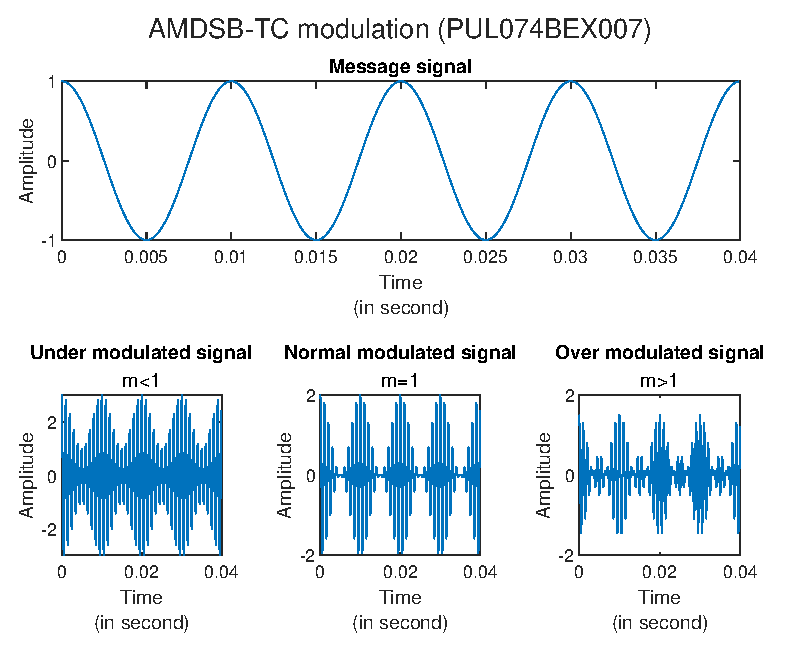
\includegraphics[width=0.8\linewidth]{../Figures/dsbtc.eps}
    \caption{DSB-TC modulation with different modulating conditions}
    \label{fig:dsbtc}
\end{figure}

\mysub{DSB-SC modulation with time and frequency domain plots}
\problem{Visualize amplitude modulation DSB-SC with the following plots.}
\subproblem{Time domain}
\subproblem{Frequency domain}

\matlabcode{amdsbsc}{Matlab script for visualization of DSB-SC modulation in time and frequency domain}
\begin{figure}[H]
    \centering
    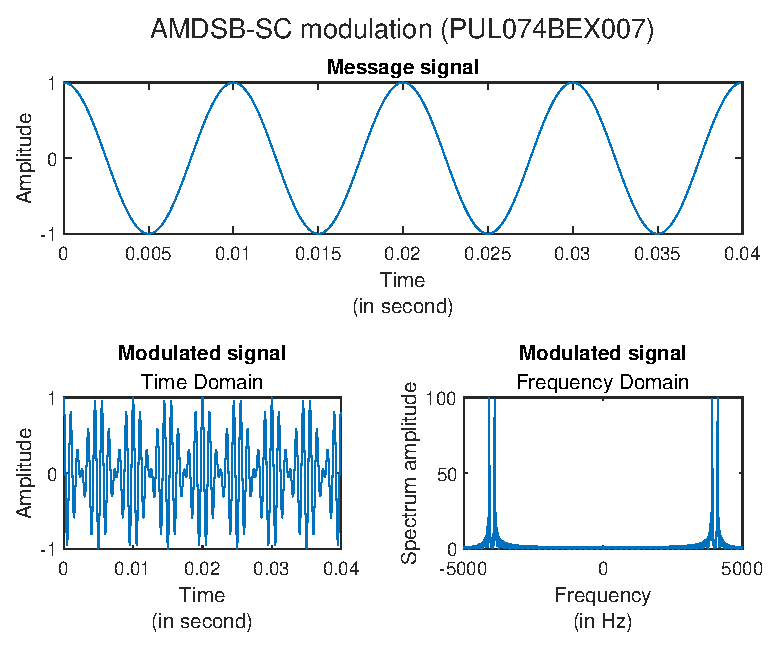
\includegraphics[width=0.8\linewidth]{../Figures/dsbsc.eps}
    \caption{DSB-SC modulation with time and frequency domain plots}
    \label{fig:dsbsc}
\end{figure}

\mysub{SSB modulation with time and frequency domain plots}
\problem{Visualize amplitude modulation SSB with the following plots.}
\subproblem{Time domain}
\subproblem{Frequency domain}

\matlabcode{amssb}{Matlab script for visualization of SSB modulation in time and frequency domain}
\begin{figure}[H]
    \centering
    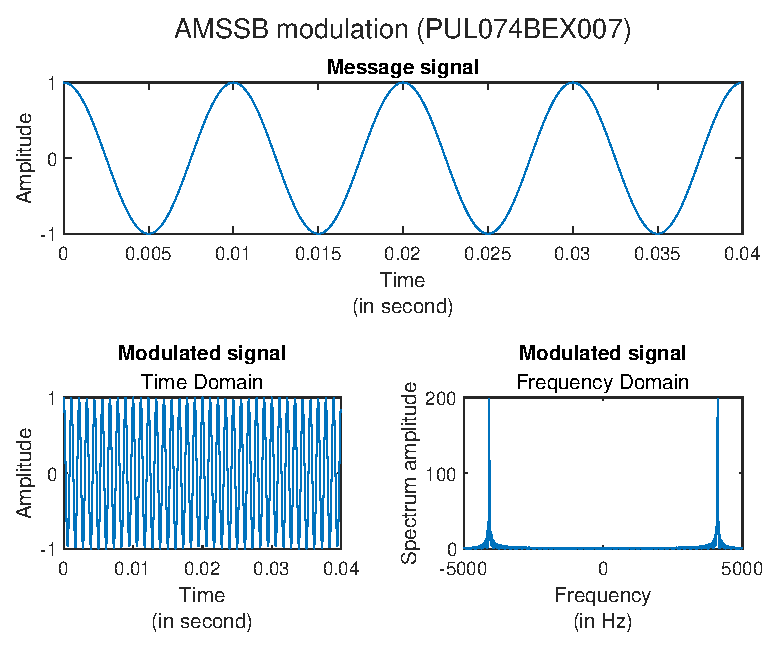
\includegraphics[width=0.8\linewidth]{../Figures/ssb.eps}
    \caption{SSB modulation with time and frequency domain plots}
    \label{fig:ssb}
\end{figure}

\pagebreak
\mysub{Demodulation of DSB-SC signal}
\problem{Visualize amplitude demodulation.}

\matlabcode{demodulation}{Matlab script for visualization of demodulation of DSB-SC signal}
\begin{figure}[H]
    \centering
    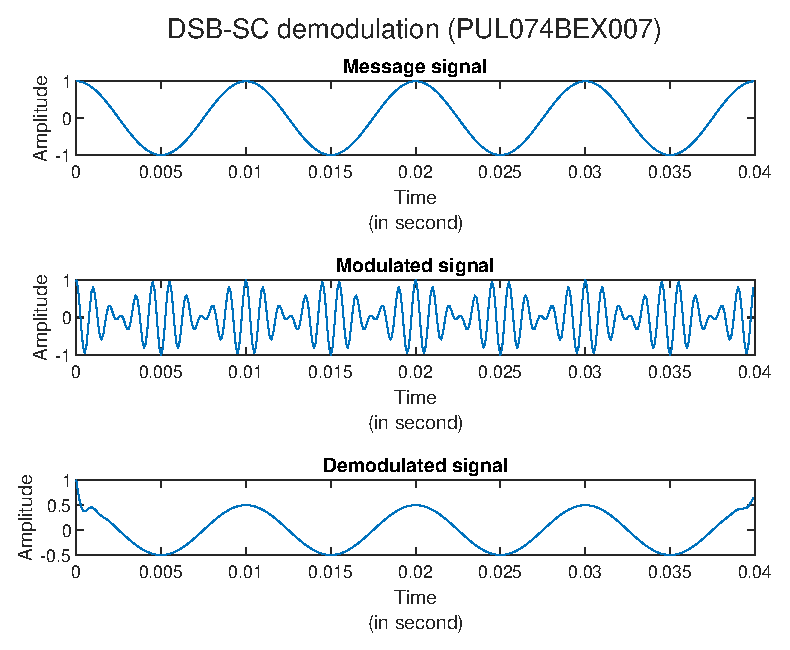
\includegraphics[width=0.8\linewidth]{../Figures/demod.eps}
    \caption{Demodulation of DSB-SC signal}
    \label{fig:demod}
\end{figure}

\section{Discussion and Conclusion}
The lab experiment dealt with the review of amplitude modulation. Double side band transmitted carrier (DSB-TC) under three modulating conditions, viz. under, normal and over modulation was visualized. Similarly, double side band suppressed carrier (DSB-SC) and single side band (SSB) modulation were plotted in time and frequency domain. Likewise, a demodulation exercise was also performed for DSB-SC signal. The objective of the lab experiment was fulfilled.
\end{document}
